% Define the type of document we want to create
\documentclass[paper=a4,media/anfibrief,fromlogo=on]{scrlttr2}

% Packages
\usepackage[utf8]{inputenc}
\usepackage[htt]{hyphenat}
\usepackage{german}
\usepackage{graphicx}
\usepackage{pdfpages}
\usepackage{xcolor}
\usepackage{eurosym}
\usepackage{graphics}
\usepackage{url} % especially useful for line breaks and online version
\PassOptionsToPackage{hyphens}{url} % avoids package loading clash with url and hyperref
\usepackage{hyperref}
\widowpenalty = 10000

\usepackage{fancyhdr}
\fancypagestyle{firststyle}
{
   \fancyhf{}
   \fancyfoot[C]{\tiny Sourcecode verfügbar unter \, \url{https://github.com/fsi-tue/anfibrief}\\ Aktuellste Version verfügbar unter \, \url{https://teri.fsi.uni-tuebingen.de/anfibrief/}\\ Revision: \gitCommit}
   \renewcommand{\headrulewidth}{0pt} % removes horizontal header line
}

% Metadata
\pdfinfo{
  /Author (Fachschaft Informatik)
  /Title  (Brief \studiengang)
  /Subject (\studiengang in Tuebingen)
  /Keywords (Erstsemester;FSI;WSI;Uni Tuebingen,Studienanfaenger;\studiengang)
}

% Beginning of the actual document
\begin{document}
  \date{\today}
  \setkomavar{subject}{\studiengang in T"ubingen }

  \begin{letter}
    {An alle Studienanfänger\\
    des Studiengangs\\
    \studiengang (\abschluss)\\
    \ifsommersemester
    Sommersemester \YEAR
    \fi
    \ifwintersemester
    Wintersemester \YEAR
    \fi
    }

    \opening{Liebe Studienanfängerin, lieber Studienanfänger,}

    \thispagestyle{firststyle}
wir freuen uns, dass du dein Studium der \studiengang in Tübingen beginnst.
Um dir den Einstieg in das Studium etwas zu erleichtern, bekommst du jetzt schon einmal
ein paar Informationen, die dir durch die ersten Wochen helfen sollen.

\ifkogwiss
\glqq Fachschaft\grqq, wer oder was ist das eigentlich? Wir, die Fachschaft Kognitionswissenschaft, 
sind eine Gruppe Studierender, die sich für die Interessen der Studierendschaft einsetzen. Zu unserer Arbeit
gehört einerseits die Vertretung der Studierenden in den Universitätsgremien, andererseits versuchen wir, unseren
Mitstudierenden das Leben an der Universität zu erleichtern (z. B. durch Ersti-Betreuung, Feste, Beratung, etc.). 
Dabei arbeiten wir eng mit der Fachschaft Informatik (fsi) zusammen.
\else
\glqq Fachschaft\grqq, wer oder was ist das eigentlich? Wir, die Fachschaft Informatik, sind eine Gruppe Studierender aus den Fächern
Informatik, Bioinformatik, Medieninformatik, Medizininformatik und Machine Learning, die sich für die Interessen der Studierendschaft einsetzen. Zu unserer Arbeit
gehört einerseits die Vertretung der Studierenden in den Universitätsgremien, andererseits versuchen wir, unseren
Mitstudierenden das Leben an der Universität zu erleichtern (z. B. durch Ersti-Betreuung, Feste, Beratung, etc.). 
Dabei arbeiten wir eng mit der Fachschaft Kognitionswissenschaften (fsk) zusammen.
\fi

Wir empfehlen sehr, an den Ersti-Veranstaltungen teilzunehmen, da 
\ifbachelor 
die Umstellung von Schulalltag auf Unialltag vielen oft schwer fällt. 
\fi
\ifmaster
die Umstellung zum Master oder dem Studium an einer neuen Uni vielen oft schwer fällt und du so bereits einen ersten Einblick in den Alltag in Tübingen erhältst.
\fi 
Bei den Veranstaltungen werden viele Studierende aus höheren Semestern anwesend sein, die dir gerne alle Fragen beantworten. 
So kannst du dir einen groben Überblick über dein Studium in Tübingen verschaffen und dabei schon die ersten Kontakte zu deinen Mitstudierenden knüpfen.
Eine Übersicht über die angebotenen Veranstaltungen findest du auf den nächsten Seiten.

Solltest du vor oder auch nach unseren Infoveranstaltungen noch Fragen haben, kannst du uns
am besten per E-Mail unter \texttt{fsi\At fsi.uni-tuebingen.de}
\ifkogwiss
sowie \texttt{kogni-fachschaft\At fsi.uni-tuebingen.de}
\fi
erreichen.
\ifkogwiss
% TODO: Ersti-Mentor*innen ändern
Zusätzlich erreichst du unsere zwei Ersti-Mentorinnen Madeleine und Laura unter der E-Mailadresse \texttt{kogni-mentoren\At fsi.uni-tuebingen.de}, die dir gerne bei Fragen rund ums erste Semester zur Verfügung stehen.
\fi
Auf unserer Website \mbox{\url{https://www.fsi.uni-tuebingen.de}} (oder \mbox{\url{https://www.fs-kogni.uni-tuebingen.de/}}) findest du bereits
jetzt viele hilfreiche Informationen rund ums Studium. Wenn du Lust hast bei der Fachschaft mitzumachen,
komm einfach zu einer unserer Sitzungen. Alle Sitzungstermine findest du auf unserer Website.
\ifkogwiss  Informationen zum Psychologie-Teil des Studiums und zu den Veranstaltungen der
Fachschaft Psychologie findest du unter \url{www.fs-psycho.uni-tuebingen.de}.\fi

Wir freuen uns schon darauf, dich bei unseren Ersti-Veranstaltungen kennenzulernen!\\
%\vfill
\ifkogwiss
Deine Fachschaften Kognitionswissenschaft und Informatik
\else
Deine Fachschaft Informatik
\hfill
{\footnotesize Redaktion: Elisa \& Linus\par}
\fi
\vfill

    %\vfill
    %PS: Wir werden aus Datenschutzgründen nicht über die Ablehnungen informiert und schicken diesen
Brief daher grundsätzlich an alle Bewerbenden. Wenn Du Deine Zulassung ablehnen willst, kannst Du diesen Brief
ignorieren -- Du würdest uns allerdings sehr helfen, wenn du uns
kurz per E-Mail über die Gründe für diese Entscheidung informierst.


    \pagebreak

% Impfkampagne
%     \noindent\makebox[\textwidth][c]{%
%     	\setlength{\fboxrule}{4pt}
%     	\fcolorbox{green}{white}{
%     		\begin{minipage}[t]{
%     				\textwidth}
%     			Solltest du noch nicht geimpft sein, hast du noch die Möglichkeit einen Termin über die Uni zu bekommen. Nutze die Chance um dich und Andere zu schützen.\\
%     			Weitere Infos findest du unter \url{https://uni-tuebingen.de/universitaet/infos-zum-coronavirus/impfen/} oder \url{https://dranbleiben-bw.de}.
%     \end{minipage}}}\vspace{0.5cm}

    \Fett{Dein Terminkalender für die ersten Tage}

    \enlargethispage{1ex}
    
% Roter Kasten mir Corona Disclaimer und anmeldung für events.
\setlength{\fboxrule}{4pt}
	\fcolorbox{red}{white}{
		\begin{minipage}[t]{
            \textwidth}
                \ifml
                    \textbf{Attention!} Due to the current situation regarding COVID-19 the dates for this semester may still change.
                    Check \textbf{in any case}~\url{https://www.fsi.uni-tuebingen.de/du-bist-ersti}, to find out the newest information.\\\\
                      % HINWEIS ZUR ANMELDUNGGame NightGILT IMMERGame NightNICHT LÖSCHEN
                    \textbf{Note:} \textbf{Please register for all events}, unless it is explicitly stated that no registration is necessary. Further details on the respective event and the registration can always be found on \url{https://www.fsi.uni-tuebingen.de/du-bist-ersti}.
                \else
                    \textbf{Achtung!} Aufgrund der aktuellen Situation können sich die Ersti-Termine für dieses Semester noch ändern.
                    Schau auf jeden Fall auf \url{https://www.fsi.uni-tuebingen.de/du-bist-ersti} nach, dort werden wir die aktuellsten Daten veröffentlichen.\\\\
                      % HINWEIS ZUR ANMELDUNGGame NightGILT IMMERGame NightNICHT LÖSCHEN
                   	\textbf{Bitte melde dich zu allen Veranstaltungen an}, außer es steht explizit dabei, dass keine Anmeldung notwendig ist. Weitere Details und die Anmeldung zur jeweiligen Veranstaltung  findest du auch immer auf \url{https://www.fsi.uni-tuebingen.de/du-bist-ersti}.
                \fi
		\end{minipage}}
\begin{description}


% Kogni Mathe Vorkurs
\ifkogwiss
    \ifmaster
        \item[Montag, 4. Oktober \YEAR, 08:00 Uhr, Ort wird noch bekannt gegeben]\ \\
        Heute beginnt der Vorbereitungskurs Mathematik speziell für Kognitionswissenschaftler im Master. Es ist zwar nicht Pflicht, daran teilzunehmen, aber sehr empfehlenswert. Nicht zuletzt lernt ihr hier erste Mitstudierende kennen! Der Vorkurs bietet euch eine Zusammenfassung des Mathestoffs, der im Bachelor Kognitionswissenschaft an der Uni Tübingen behandelt wird.
        \textbf{Wenn ihr euren Bachelor nicht an der Universität Tübingen oder in einem anderen Fach erworben habt, kann der Vorkurs für euch sinnvoll sein.} Falls ihr Quereinsteiger seid, werdet ihr dadurch an die in eurem Studium benötigten mathematischen Grundlagen herangeführt. Falls ihr bereits mathematisches Vorwissen mitbringt, ist der Kurs eine gute Gelegenheit, euer Wissen aufzufrischen.\\
         Es wäre super, wenn ihr euch mit einer kurzen Mail an \texttt{kogni-beratung@fsi.uni-tuebingen.de} bei Simon Mustermann anmelden würdet. Als Treffpunkt für Montag den 04. Oktober könnt ihr euch am Eingang des Psychologischen Instituts einfinden. Alle weiteren Infos erhaltet ihr dann per Mail.\\

%Stattfinden wird der Vorkurs im ÜR 08 in der alten Physik, das ist die Gmelinstraße 6. Diese befindet sich an der Bushaltestelle Gmelinstraße, nördlich gegenüber von der Neuen Aula. Wenn ihr auf der Wilhelmstraße seid, geht rechts an der Neuen Aula vorbei, dort findet ihr die Alte Physik an der Ecke Gmelin- und Nauklerstraße, rechts von der Neuen Aula. Seid ihr auf der Hölderlinstraße, geht links dran vorbei und die Alte Physik ist auf der linken Straßenseite. Genaue Informationen bezüglich Treffpunkt am ersten Termin erhaltet ihr dann nochmal per Mail.
%
%\seticon{faBus}~\textbf{Bushaltestelle:} Gmelinstraße, Hölderlinstraße, Uni/Neue Aula
%
%\else
    \fi
\fi

\ifml
	\item~ % Funktioniert nicht anders, don't judge me
\else
	% Mathe-Vorkurs
    \item[Mathevorkurs - \mathedatum~\YEAR]~\\
    \ifbachelor
    Heute beginnt der Vorbereitungskurs Mathematik. Es ist zwar nicht Pflicht, daran teilzunehmen, aber es ist sehr empfehlenswert.
    \fi
    \ifmaster
    Wenn du deinen Bachelor nicht in Tübingen oder in einem mathefremden Fach erworben hast, kann dieser Vorkurs für dich sehr sinnvoll sein. Auf unserer Website findest du ein Skript mit den Inhalten des Vorkurses. Damit solltest du einschätzen können, wie viel vom Stoff bereits bekannt ist und ob sich der Besuch des Vorkurses lohnt.\\\\
    \fi
	Der Vorkurs bietet dir eine Wiederholung des Schulstoffes und eine Einführung in die Uni-Mathematik. Zudem hast du die Möglichkeit, einige deiner neuen Mitstudierenden kennenzulernen und erste Lerngruppen zu bilden.
	
	\textbf{Anmeldeschluss:} \matheanmeldung\YEAR\\
	Anmeldung/Infos unter:  \url{https://uni-tuebingen.de/de/91877}\\
	Kontakt: \texttt{janosch.doecker\At uni-tuebingen.de}\\
	\ifsommersemester
	\seticon{faBus}~\textbf{Bushaltestelle:} Sand Drosselweg (Linien 2 \& 6) 
	\fi
\fi

\ifmaster
    \ifbinfo
        \item[Informatikvorkurs - \bioinfoDatum~\YEAR]\ \\
            Heute beginnt ein Informatik-Vorkurs speziell für Bioinformatik-Studierenden (Variante B) im Master. Dieser Vorkurs wird dringend empfohlen, wenn du aus einem fachfremden Studiengang wie z.B. Biologie oder anderen Lebenswissenschaften kommst und nur wenig Erfahrung in der Informatik und der Programmierung (CLI, Java, Python, \LaTeX) hast. Der Vorkurs wird in Englisch gehalten. \\
            \textbf{Anmeldeschluss:} \bioinfoAnmeldung\YEAR\\
            Anmeldung/Infos unter: \url{https://uni-tuebingen.de/de/91881}\\
            Kontakt: \texttt{philipp.thiel\At uni-tuebingen.de}\\
        \seticon{faBus}~\textbf{Bushaltestelle:} Sand Drosselweg (Linien 2 \& 6)
    \fi
\fi

%%%%%%%%%%%%%%%%%%%%%%%%%%%%%%%%%%%%%%%%%%%%%%%%%%%%%%%%%%%%%%%%%%%%%%%%%%%%
% Ab hier die FSI Events einfügen. Darüber sind der Mathe und Info vorkurs.

% Kastenlauf
\ifml
	\item[Crate Run - Friday, October 7th, \YEAR, 19:00, Sand]~\\
	\seticon{faBus}~\textbf{bus stop:} Sand Drosselweg (bus lines 2 \& 6)
\else
	\item[Kastenlauf - Freitag, 7. Oktober \YEAR, 19 Uhr, Sand]~\\

	\seticon{faBus}~\textbf{Bushaltestelle:} Sand Drosselweg (Linien 2 \& 6)
\fi


%Spieleabend 1
\ifml
	\item[Board Game Night 1 - Thursday, October 13th, \YEAR, 19:00, Sand]~\\
	We'd like to invite you to a board game night in relaxed atmosphere at the Sand.
    We'll provide some games as well as drinks and snacks (for a small donation).
    Even though our collection is growing steadily, we're more than happy if you bring along your own games!\\
	\seticon{faBus}~\textbf{bus stop:} Sand Drosselweg (bus lines 2 \& 6)
\else
    \item[Spieleabend 1 - Donnerstag, 13. Oktober \YEAR, 19 Uhr, Sand]~\\
	Wir möchten dich zu einem kleinen Analog-Spieleabend mit guter Gesellschaft und entspannter Atmosphäre auf dem Sand einladen.
    Für einige Spiele sowie Getränke und Knabberkram (gegen einen kleinen Obolus) sorgt die Fachschaft.
    Wir freuen uns natürlich sehr, wenn du auch eigene Spiele mitbringst, obwohl unsere Sammlung schon beachtlich ist!\\
	\seticon{faBus}~\textbf{Bushaltestelle:} Sand Drosselweg (Linien 2 \& 6)
\fi

% Frühstück
% TODO: Lisbeth fragen, wer Zeilgruppe ist
\ifbachelor
	\item[Frühstück - Freitag, 11. Oktober \YEAR, 9 Uhr, Mensa Morgenstelle]\ \\
	Wir laden dich an diesem Morgen zu einem gemütlichen Frühstück ein! Dabei erfährst du einiges über die Uni, die Fachschaft und was dich in den nächsten Monaten erwartet - auch im Gespräch mit älteren Studierenden.
	Danach machen wir eine Führung über die Morgenstelle, damit du die wichtigsten Räume und Hörsäle kennen lernst.
	Wenn du Lust hast, kannst du anschließend ab 11:45 Uhr das Mensaessen ausprobieren.\\
	\seticon{faBus}~\textbf{Bushaltestelle:} BG Unfallklinik (Linien 5, 13, 14, 17, 18, 19, X15)
\fi

%Wanderung
\ifml
	\item[Hike - Saturday, October 15th \YEAR, 11:00, in front of Neckarmüller]~\\
	On a leisurely hike you will get to know not only your fellow students,
	but also a few lecturers and the worthwhile surroundings of Tübingen!
	The meeting point is at the Neckarbrücke \emph{in front of the} restaurant \glqq Neckarmüller\grqq.
	\seticon{faBus}~\textbf{bus stop:} Neckarbrücke (lines 1-22)
\else
	\item[Wanderung - Samstag, 15. Oktober \YEAR, 11 Uhr, vor dem Neckarmüller]~\\
	Bei einer gemütlichen Wanderung lernt ihr neben euren Kommilitonen und Kommilitoninnen auch
	noch ein paar Dozierende und die sehenswerte Tübinger Umgebung kennen!
	Der Treffpunkt ist bei der Neckarbrücke (\emph{vor} dem Gasthaus \glqq Neckarmüller\grqq).\\
	\seticon{faBus}~\textbf{Bushaltestelle:} Neckarbrücke (Linien 1-22) 
\fi

%Stadtrallye
\ifml
	\item[City Rally - Tuesday, October 18h \YEAR, 16:00 Uhr, \footnotesize{location \& start time will be given to you after registration}]~\\
	On this evening, you can participate in a team-based scavenger hunt across the city,
	where you will get to know interesting, beautiful as well as disturbing spots within Tübingen.
	As a side effect, you will hopefully get to know your new home town a bit better and make new friends.
\else
	\item[Stadtrallye - Dienstag, 18. Oktober \YEAR, 16 Uhr, \footnotesize{Ort \& Zeit wird dir nach Anmeldung mitgeteilt}]\ \\
	Bei der Stadtrallye lassen wir dich und deine Kommilitonen und Kommilitoninnen gegeneinander in Teams antreten.
	Dabei werdet ihr interessante, schöne und verstörende Ecken Tübingens kennenlernen.
\fi


% Kneipentour
\ifml
\item[Pub Crawl - Wednesday, April 19th \YEAR, 18:00, \footnotesize{location \& start time will be given to you after registration}]~\\
Tübingen is laced with small bars and pubs that have a significant impact on the night life in Tübingen.
In order to calm down from the stress of this information-filled day, we'd like to invite you to go bar-hopping with us.
We'll divide up into small groups and visit the different bars in the historic town center.
Please bring enough cash, most places we will visit don't accept cards (\emph{none whatsoever}).

\else
\item[Kneipentour - Mittwoch, 19. April \YEAR, 18 Uhr, \footnotesize{Ort \& Zeit wird dir nach Anmeldung mitgeteilt}]~\\
Tübingen ist übersät mit kleinen Kneipen und Bars, die das Nachtleben maßgeblich bestimmen.
Um den Stress der ersten Veranstaltungen etwas sacken zu lassen, laden wir dich zu einer ausgiebigen Kneipentour ein,
bei der wir in Kleingruppen die verschiedenen Lokalitäten der Tübinger Altstadt besuchen.
Bitte bringe genügend Bargeld mit, man kann in fast keiner der Tübinger Bars mit EC-Karte zahlen! -- Volksbanken und Sparkassen finden sich bei Bedarf in der Stadt.
\fi

%Grillen
\ifml
	\item[BBQ - Saturday, October 22th \YEAR, 17:00, Sand 13, garden]~\\
	You're not in the mood for cooking this evening? Fear not!
    The student council invites you for a BBQ. Bring whatever you want to put on the grill,
    please also bring your own plates and cutlery. The garden has enough space for stuff like volleyball, football etc. as well.\\
	\seticon{faBus}~\textbf{bus stop:} route 2, route 6, Sand Drosselweg
\else
	\item[Grillen - Samstag, 22. Oktober \YEAR, 17 Uhr, im Garten des Sandes]~\\
	Du hast keinen Bock auf Kochen? Dann bist du hier genau richtig! In geselliger Runde wird die Fachschaft mit dir grillen.
	Bring dazu mit, was auch immer du zum Grillen brauchst, Gas- und Kohlegrill warten auf dich. Vergiss bitte auch nicht, dein Besteck und Geschirr einzupacken!\\
	Auf dem Sand ist es auch möglich Volleyball, Fußball, usw. zu spielen. Wir freuen uns auf dich!
	\seticon{faBus}~\textbf{Bushaltestelle:} Sand Drosselweg (Linien 2 \& 6)
\fi

% Nur damit die seite richtig gebrochen wird. 
% Muss jedes jahr angepasst werden.
\ifbachelor
\pagebreak
\fi


%Spieleabend 2
\ifml
	\item[Board Game Night - Thursday, October 27th, \YEAR, 19:00, Sand]\ \\
	We'd like to invite you to a board game night in relaxed atmosphere at the Sand.
	We'll provide some games as well as drinks and snacks (for a small donation).
	Even though our collection is growing steadily, we're more than happy if you bring along your own games!\\
	\seticon{faBus}~\textbf{bus stop:} Sand Drosselweg (bus lines 2 \& 6)
\else
    \item[Spieleabend 1 - Donnerstag, 13. Oktober \YEAR, 19 Uhr, Sand]~\\
	Wir möchten dich zu einem kleinen Analog-Spieleabend mit guter Gesellschaft und entspannter Atmosphäre auf dem Sand einladen.
	Für einige Spiele sowie Getränke und Knabberkram (gegen einen kleinen Obolus) sorgt die Fachschaft.
	Wir freuen uns natürlich sehr, wenn du auch eigene Spiele mitbringst, obwohl unsere Sammlung schon beachtlich ist!\\
	\seticon{faBus}~\textbf{Bushaltestelle:} Sand Drosselweg (Linien 2 \& 6)
\fi

%KOGWIS
\ifkogwiss
% Bus-Schnitzeljagd, neu im WS19/20
\item[Bus-Schnitzeljagd - Samstag, 31. Oktober \YEAR, mit Anmeldesystem]\ \\
    Bei der Schnitzeljagd wirst du mit deinen Kommilitonen in Teams losgeschickt, um das Tübinger Busnetz zu erkunden. Durch das Lösen verschiedener Rätsel lernt ihr dabei nicht nur eure neuen Kommilitonen sondern auch einige Haltestellen besser kennen, die euch in eurem Uni-Alltag mehr oder weniger häufig begegnen werden. Da Studenten in Tübingen (und im kompletten naldo-Bereich) montags bis freitags ab 19:00 Uhr sowie ganztägig an Samstagen, Sonntagen und gesetzlichen Feiertagen in Baden-Württemberg kostenlos Bus und Bahn fahren dürfen, benötigt ihr für eure Erkundungstour lediglich euren Studierendenausweis.\\
    Für die Durchführung planen wir ein Anmeldesystem, um die Gruppen gestaffelt losschicken zu können. Dieses findest du über einen Link auf unserer Fachschafts-Website \url{https://www.fs-kogni.uni-tuebingen.de/}.
    Falls sich Details ändern sollten, findest du weitere Infos wie Uhrzeit und Treffpunkt ebenfalls auf unserer Webseite oder auf der Website der Fachschaft Informatik \url{https://www.fsi.uni-tuebingen.de/ersti}.\\
\fi

\ifkogwiss
\item[Vorstellung der Lehrstühle - Montag, 17. Oktober \YEAR, 16:00 Uhr und online]\ \\
    Hier stellen sich die kognitionswissenschaftlichen Lehrstühle (also die verschiedenen Forschungsbereiche der Professoren) vor. Dies ist super um einen Überblick zu bekommen, was die Kognitionswissenschaft alles beinhaltet und um erste Eindrücke von den Profs zu bekommen. Auch die Fachschaft stellt sich dir hier erstmals vor. %Danach gibt es noch Gelegenheit, mit der Fachschaft ein Glas Milch trinken zu gehen.
    Auch für Kogni-Master ist das eine super Veranstaltung. \\
    Falls sich auf Grund der aktuellen Situation Details ändern sollten, findest du weitere Infos auf der Website \url{https://www.fs-kogni.uni-tuebingen.de/}.
    
\fi

\ifkogwiss
    \item[Spiele- und Grillabend - Mittwoch, 18. Oktober, \YEAR, 20:00 Uhr und Ort Sand 14]\ \\
         Damit man sich auch unter den Kognis kennenlernen kann, veranstalten wir einen Spiele- und Informationsabend für die Kogni-Erstis. Dabei werden auch einige höhersemestrige Kognis und Fachschaftler da sein, die man zum Kogni-Studium ausfragen kann. Bei gutem Wetter werden wir möglichst draußen sitzen und uns so der aktuellen Situation anpassen. Wir hoffen, dass wir zusammen einen schönen Abend verbringen können. Kogni-Master sind natürlich auch herzlich eingeladen.
         %Hier können Gesellschaftsspiele und bei gutem Wetter auch Tischtennis und Volleyball gespielt werden. Für Verpflegung können wir leider nicht auf eigene Kosten sorgen aber wir stellen gegen eine kleine Spende Getränke bereit und bestellen Pizza. Es werden auch einige höhersemestrige Kognis und Fachschaftler da sein, die man zum Kogni-Studium ausfragen kann. Kogni-Master sind natürlich auch herzlich eingeladen.
	\seticon{faBus}~\textbf{Bushaltestelle:} Linie 2, Sand Drosselweg (Rest ausgeschildert)
	Falls sich auf Grund der aktuellen Situation Details ändern sollten, findest du weitere Infos auf der Website \url{https://www.fs-kogni.uni-tuebingen.de/}.
\fi


% erste Vorlesung (TODO ohne corona wieder reinnehmen)
%\ifbachelor
%\item[Dienstag, 14. April \YEAR, Morgenstelle, Hörsaal N7]\ \\
%Deine erste Vorlesung beginnt um
%\ifwintersemester 8 Uhr -- Du hast „Mathe I für Informatiker“  \fi
%\ifsommersemester 10 Uhr -- Du hast „Mathe II für Informatiker“  \fi
%bei \Matheprof.
%Alles, was du heute (und in Zukunft) benötigst: persönlichen Wachmacher, einen Stift, einen Block und den Studierendenausweis.

%\seticon{faBus}~\textbf{Bushaltestelle:} BG Unfallklinik (Linie 5, 13, 14, 17, 18, 19, X15)
%\fi

%Clubhausfest
\ifml
    \item[Clubhausfest - Thursday, November 3rd \YEAR, 21:00, Clubhaus]\ \\
        Every thursday during the lecture period, a different student body or group of students organizes the "`Clubhaus Fest"' in the Clubhaus, which locates directly opposite of the new auditorium. Today the attendance is particularly worthwhile, because the student councils of computer science, cognitive science and psychology are hosting the event! 

        \seticon{faBus}~\textbf{bus stop:} Uni/Neue Aula or Hölderlinstraße
\else
    \item[Clubhausfest - Donnerstag, 3. November \YEAR, 21:00 Uhr, Clubhaus]\ \\
        Während der Vorlesungszeit richtet jeden Donnerstag eine andere Fachschaft oder studentische Gruppierung das Clubhausfest im Clubhaus, direkt gegenüber der Neuen Aula, aus. Heute lohnt sich der Besuch jedoch ganz besonders, denn die Fachschaften Informatik, Kogni und Psychologie sind Gastgeber!
%Das anfängliche Chaos des Vorlesungsbeginns hat sich gelegt und auch an diesem Donnerstag findet das Clubhausfest statt.

%\seticon{faBus}~\textbf{Bushaltestelle:} Uni/Neue Aula bzw. Hölderlinstraße
\fi

\ifkogwiss
    \item[Montag, 8. Oktober \YEAR, 17 Uhr, Sand Terasse ]\ \\
    Damit sich die Kognis untereinander kennenlernen, gibt es einen Abend nur für diese. Der genaue Ablauf des Abends wird im Laufe der ersten Vorkurswoche bekannt gegeben.
\fi

%Ersti-Mentorenprogramm
\ifbachelor
	\item[TBA] Dieses Semester bietet unser Fachbereich speziell ein Mentoren-Programm für Erstis an. Dabei soll es ein regelmäßiges Treffen zwischen einem Professor und Kleingruppen an Studenten geben, in denen Fragen und Probleme geklärt werden. Weitere Details folgen.
\fi

\end{description}

    \pagebreak
    
    \Fett{Das erwartet dich im Studium} \\
    \fett{Stundenplan}
    \input{stundenplaene/stpl_\Timetable}
    %TODO Nächstes Semester: Anpassen
    \iflehramt \ifbachelor \newpage \fi \fi
    ~\\

\fett{Die wichtigsten Online-Portale}
Um keine wichtigen Informationen zu verpassen, solltest du dich mit den Online-Lehrportalen der Uni Tübingen vertraut machen
\footnote{Ja, wir sprechen bewusst in der Mehrzahl, denn wo und wie Lehrmaterialien und Informationen veröffentlicht werden, ist leider immer noch 
von Lehrstuhl zu Lehrstuhl unterschiedlich und man findet sich bei so manchem Modul in einer stattlichen Link-Sammlung wieder.}.
\begin{itemize}
	\item \textbf{\hypertarget{alma}{alma}} \url{https://alma.uni-tuebingen.de/} \\
	alma ist das zentrale Vorlesungsverzeichnis der Uni Tübingen. Es ist der Startpunkt, von dem aus du dich auf das tatsächlich verwendete Portal weiterleiten lässt.
	Hier findest du alle angebotenen Veranstaltungen des ausgewählten Semesters. Unter \texttt{Studienangebot > Vorlesungsverzeichnis anzeigen} kannst du dir die Vorlesungen heraussuchen. Die Prüfungsanmeldung gegen Ende des Semesters erfolgt meist auch über alma.  
	\item \textbf{Ilias} \url{https://ovidius.uni-tuebingen.de/} \\
	Ilias bietet verschiedene Kommunikationstools an und ist das am häufigsten verwendete Portal, um eine Vorlesung zu organisieren. Auch hier könnt ihr einzelne Veranstaltungen suchen, jedoch empfehlen wir, zuerst bei alma reinzuschauen. 
	\item Zusätzlich gibt es dann noch eigene Foren, Teaching Websites bis hin zu Discord Servern, auf die du aber allesamt über die beiden Portale oben weitergeleitet wirst, falls sie verwendet werden.
	
\end{itemize}
\fett{Die Anfangszeiten und Orte}
Wie du sicher bald bemerken wirst: 9 Uhr heißt 9.15 Uhr. An der Uni fangen Veranstaltungen in der Regel c.t. (\textit{cum
tempore}, lat. \glqq mit Zeit\grqq) an. Wenn etwas „pünktlich“ anfängt, wird es als s.t. (\textit{sine tempore}, lat. \glqq ohne
Zeit\grqq) angekündigt.
Bezüglich der genauen Zeiten und Orte solltest du vor Vorlesungsbeginn unbedingt Blick in das \hyperlink{alma}{alma}-Portal werfen.


\ifbachelor
\fett{Die ersten Vorlesungen}
\begin{itemize}
	\item 
	\textbf{Die Informatik-Vorlesung} \\
	Die 
	\ifwintersemester Informatik I \fi
	\ifsommersemester Informatik II \fi 
	ist eine gründliche Einführung in die Entwicklung von Programmen und die dazugehörigen formalen Grundlagen. 
	Du verbringst einen Großteil der Zeit damit, eigene Programme zu schreiben und wirst dabei Schritt für Schritt 
	an Konzepte wie Rekursion oder Abstraktion herangeführt. 
	\ifwintersemester In der Informatik I wird dazu die funktionale Programmiersprache DrRacket verwendet. \fi
	\ifsommersemester Die Vorlesung Informatik II ist unabhängig von der Informatik I und kann auch zu Beginn gehört werden. \fi
	%\fett{Die Informatik-Vorlesung}
	%Die Vorlesung Informatik II ist unabhängig von der Informatik I und bietet euch einen Einstieg
	%in ein vielen noch unbekanntes Thema, die funktionale Programmierung. Im Zentrum stehen dabei Techniken der Abstraktion von Teilproblemen, um den Ablauf komplexerer Programme im Kern zu verstehen und somit Fehler beim Programmieren besser vermeiden zu können.
	
	\ifinfo
	\ifwintersemester
	\item 
	\textbf{Technische Informatik} \\
	In \glqq Einführung in die Technische Informatik\grqq \ lernt ihr von den physikalischen Basics bis hin zu Dioden und Transitoren alle notwendigen Grundlagen, um die Funktionsweise von Computern zu verstehen. Auch wenn die Informatik oder Mathematik scheinbar wichtiger sind, solltet ihr hier immer am Ball bleiben! Die Vorlesung basiert weitestgehend auf dem Buch \glqq Technische Informatik\grqq \ von Wolfram Schiffmann.
	\fi
	\fi
	
	\item 
	\textbf{Die geliebte Mathematik} \\
	Die Mathe-Vorlesungen gehören zu den Herausforderungen der ersten Semester und du wirst merken, dass in der Uni-Mathematik ein sehr großer Teil an Selbststudium von dir erwartet wird. Die Vorlesungen orientieren sich an dem Lehrbuch: „Mathematik für Informatiker und Bioinformatiker“ von Prof. Hauck, Prof. Wolff und Prof. Küchlin. Eine gute Möglichkeit zur Einstimmung bietet der „Mathematische Vorbereitungskurs für das Studium der Informatik“ (siehe oben). 
	\iflehramt
	Mathematik-Studenten brauchen Mathematik I
	und II nicht besuchen, da diese Module durch Analysis und Lineare Algebra
	abgedeckt werden. (Weitere Informationen dazu finden sich in der
	Prüfungsordnung.).
	\fi
\end{itemize}
\fi


% Nur damit die seite richtig gebrochen wird. 
% Muss jedes jahr angepasst werden.
\iflehramt
\pagebreak
\fi

    \fett{Mailinglisten}
Es gibt mehrere Mailinglisten damit wichtige Informationen bei dir ankommen.\\
Eine vollständige Auflistung findest du unter: \url{https://www.fsi.uni-tuebingen.de/mailinglisten/}
\begin{itemize}
\item \textbf{info-studium}: \textcolor{red}{\textbf{Eine Anmeldung ist verpflichtend.}} Dies ist die einzige Möglichkeit unter der die Professorenschaft dich erreichen kann! \\
Anmeldung unter: \url{https://www.fsi.uni-tuebingen.de/mailman/listinfo/info-studium}.
\iflehramt
\item \texttt{info-lehramt}: Für alle Lehrämtler gibt es eine zusätzliche Liste. Hierüber erhaltet ihr Informationen z.B. zu Fachdidaktik und anderen lehramtsspezifischen Veranstaltungen.\\
Anmeldung unter: \url{https://www.fsi.uni-tuebingen.de/mailman/listinfo/info-lehramt}.
\fi
\ifkogwiss 
\item \texttt{kogwiss}: Eine Mailingliste für Themen, die ausschließlich Kognitionswissenschaftler betreffen. \\
Anmeldung unter: \url{https://www.fsi.uni-tuebingen.de/mailman/listinfo/kogwiss}.

\item \texttt{versuche}: Für die Suche nach Teilnehmern für Studien und Versuche (nützlich für Versuchspersonenstunden\footnote{oft abgekürzt mit VP}).\\
Anmeldung unter: \url{https://www.fsi.uni-tuebingen.de/mailman/listinfo/versuche}. 
\fi
\item \texttt{info-talk}: Diese Liste ist für Themen, die nicht direkt mit dem Studium zu tun haben, aber dennoch von Interesse sein können.\\
Anmeldung unter: \url{https://www.fsi.uni-tuebingen.de/mailman/listinfo/info-talk}.
\item \texttt{info-jobs}: Für bezahlte Angebote von HiWi\footnote{wissenschaftliche/studentische Hilfskraft}-Jobs, Praktika sowie  Werksstudentenjobs.\\
Anmeldung unter: \url{https://www.fsi.uni-tuebingen.de/mailman/listinfo/info-jobs}.
\item \texttt{coding}: Hackathons und andere Veranstaltungen zum Coden.\\
Anmeldung unter: \url{https://www.fsi.uni-tuebingen.de/mailman/listinfo/coding}.
\item \texttt{sport}: Falls ihr zu den *-Informatikern gehört, die entgegen dem Klischee gerne Sport treiben, sei euch die Liste \texttt{sport} ans Herz gelegt.\\
Anmeldung unter: \url{https://www.fsi.uni-tuebingen.de/mailman/listinfo/sport}. 
\end{itemize}

    \pagebreak
    \ifml
    \fett{Public transport in Tübingen}
    Bus schedules can be found online\footnote{\url{https://naldo.de/}} and in the Naldo app for Android and iOS.\\
    The best way to get to the "`Morgenstelle"' (see city map on the last page) is to take the bus (destination stop BG-Unfallklinik\footnote{\textbf{not} "`Auf der Morgenstelle"'!}). There is a very limited number of parking lots at the Morgenstelle, but one has to apply for a permission to use them, first.
    Most Master events/lectures take place on the "`Sand"', the place of the WSI (Wilhelm-Schickard-Institut). To get to the Sand, take line 2, stop \emph{Sand Drosselweg}. It is also easily reached by car as there are multiple parking lots.
    Some Machine Learning lectures take place in the Maria-von-Linden-Straße 6. To get there, take line 3, stop \emph{Maria-von-Linden-Straße}.
    With your semester fee you have already paid part of the semester ticket for the bus (in addition to the student union fee and the matriculation fee).
    The semester ticket costs \ticketpreis~EUR and is valid in the whole Naldo area, a public transport system around
    Tübingen (unfortunately not to Stuttgart, but to Überlingen at Lake Constance). The ticket is valid from 1 October and is available in the DB travel centres and online\footnote{\url{https://tickets.naldo.de/}}. In order to buy the semester ticket offline, you will need to show your student ID and the Semester Ticket Certificate from the data control sheet. For the online purchase you need a login ID of the university (starting with \texttt{zx}).\\
    Naldo's leisure time regulations do also apply: Here you can use buses and trams within the Naldo area free of charge on weekdays from 7 p.m. and all day on weekends. All you need is your student card with the Naldo logo on it.
    Especially interesting if your parents are visiting Tübingen: On Saturdays you can take a free bus in the city area (tariff level 11)\footnote{At least at the time of the editorial deadline this regulation still applies}, no matter if you are studying or not.\\ \\

    \fett{Housing in Tübingen}
    Unfortunately, the topic of housing has not lost its explosive power in Tübingen in recent years,
    so that it may be difficult to find accommodation. We recommend the following two Studierendenwerke as your first points of contact:
    Application forms for a place in a hall of residence can be obtained from either the Studierendenwerk AdöR in the administration of the dormitory,
    Fichtenweg 5, 72076 Tübingen, or at the Studierendenwerk e.V., Rümelinstraße 8, 72070 Tübingen. For the private housing market, Wednesday and Saturday
    editions of the Schwäbisches Tagblatt are available.
    On the Internet the platform \url{www.wg-gesucht.de} is your best option.
    You can find more information on our homepage at \url{https://www.fsi.uni-tuebingen.de/erstsemester-faq/}.

\else

    \fett{Verkehr in Tübingen}
    Die Fahrpläne für den ÖPNV  findest du online\footnote{\url{https://naldo.de/}} und in der Naldo-App für Android und iOS.\\
    Die Bushaltestelle für die Unigebäude an der \emph{Morgenstelle} (siehe Stadtplan auf der letzten Seite) heißt "`BG-Unfallklinik"'\footnote{\textbf{nicht} "`Auf der Morgenstelle"'!}). Es gibt zwar auch Parkplätze dort,
    jedoch muss man deren Benutzung beantragen und die Anzahl an Parkplätzen ist ohnehin sehr begrenzt.
    \ifmaster
    Die meisten Master-Veranstaltungen finden auf dem \emph{Sand}, dem Sitz des WSI (Wilhelm-Schickard-Institut), statt. Die Bushaltestelle heißt "`Sand Drosselweg"'.
    \fi
    Das Semesterticket kostet \ticketpreis~EUR und gilt im ganzen Naldogebiet, dem Verkehrsverbund rund um Tübingen (leider nicht bis Stuttgart, dafür bis Überlingen am Bodensee). Das Ticket gilt ab dem 
    \ifwintersemester
    1. Oktober
    \fi
    \ifsommersemester
    1. April
    \fi 
    und ist in den Reisezentren der DB und online\footnote{\url{https://tickets.naldo.de/}} erhältlich. Für den Online-Kauf benötigt ihr eine Login-ID der Uni (beginnend mit \texttt{zx}). Falls ihr das Semesterticket offline kaufen möchtet, müsst ihr euren Studiausweis sowie die "`Bescheinigung für das Semesterticket"' vom Datenkontrollblatt vorzeigen. \\
    Außerdem gilt die Freizeitregelung von Naldo: Hier könnt ihr unter der Woche ab 19 Uhr und am Wochenende ganztägig Busse und Bahnen innerhalb des Naldo-Gebiets kostenlos nutzen. Dafür braucht ihr einfach nur euren Studiausweis, auf dem sich das Naldo-Logo befindet.
    Besonders interessant, falls die Eltern zu Besuch in Tübingen sind: Samstags kann man im Stadtgebiet (Tarifstufe 11) kostenlos Bus fahren\footnote{Zumindest zum Zeitpunkt des Redaktionsschlusses gilt diese Regelung noch}, egal ob man studiert oder nicht. \\\\

    \fett{Wohnen in Tübingen}
    Das Thema Wohnen hat in Tübingen in den letzten Jahren leider nicht an Brisanz verloren, so dass
    es unter Umständen schwierig ist, eine Unterkunft zu finden. Als erste Anlaufstellen empfehlen wir
    die beiden Studierendenwerke: Antragsformulare für einen Wohnheimplatz gibt es entweder beim
    Studierendenwerk AdöR in der Wohnheimverwaltung, Fichtenweg 5, 72076 Tübingen, oder beim Studierendenwerk
    e.V., Rümelinstraße 8, 72070 Tübingen. Für den privaten Wohnungsmarkt sind Mittwochs- und Samstagsausgabe
    des Schwäbischen Tagblatts zu empfehlen.
    Im Internet hat sich \url{www.wg-gesucht.de} etabliert. Mehr gibt es auf unserer Homepage unter \url{https://www.fsi.uni-tuebingen.de/erstsemester-faq/}.
    \fi

    \vfill
    \pagebreak
    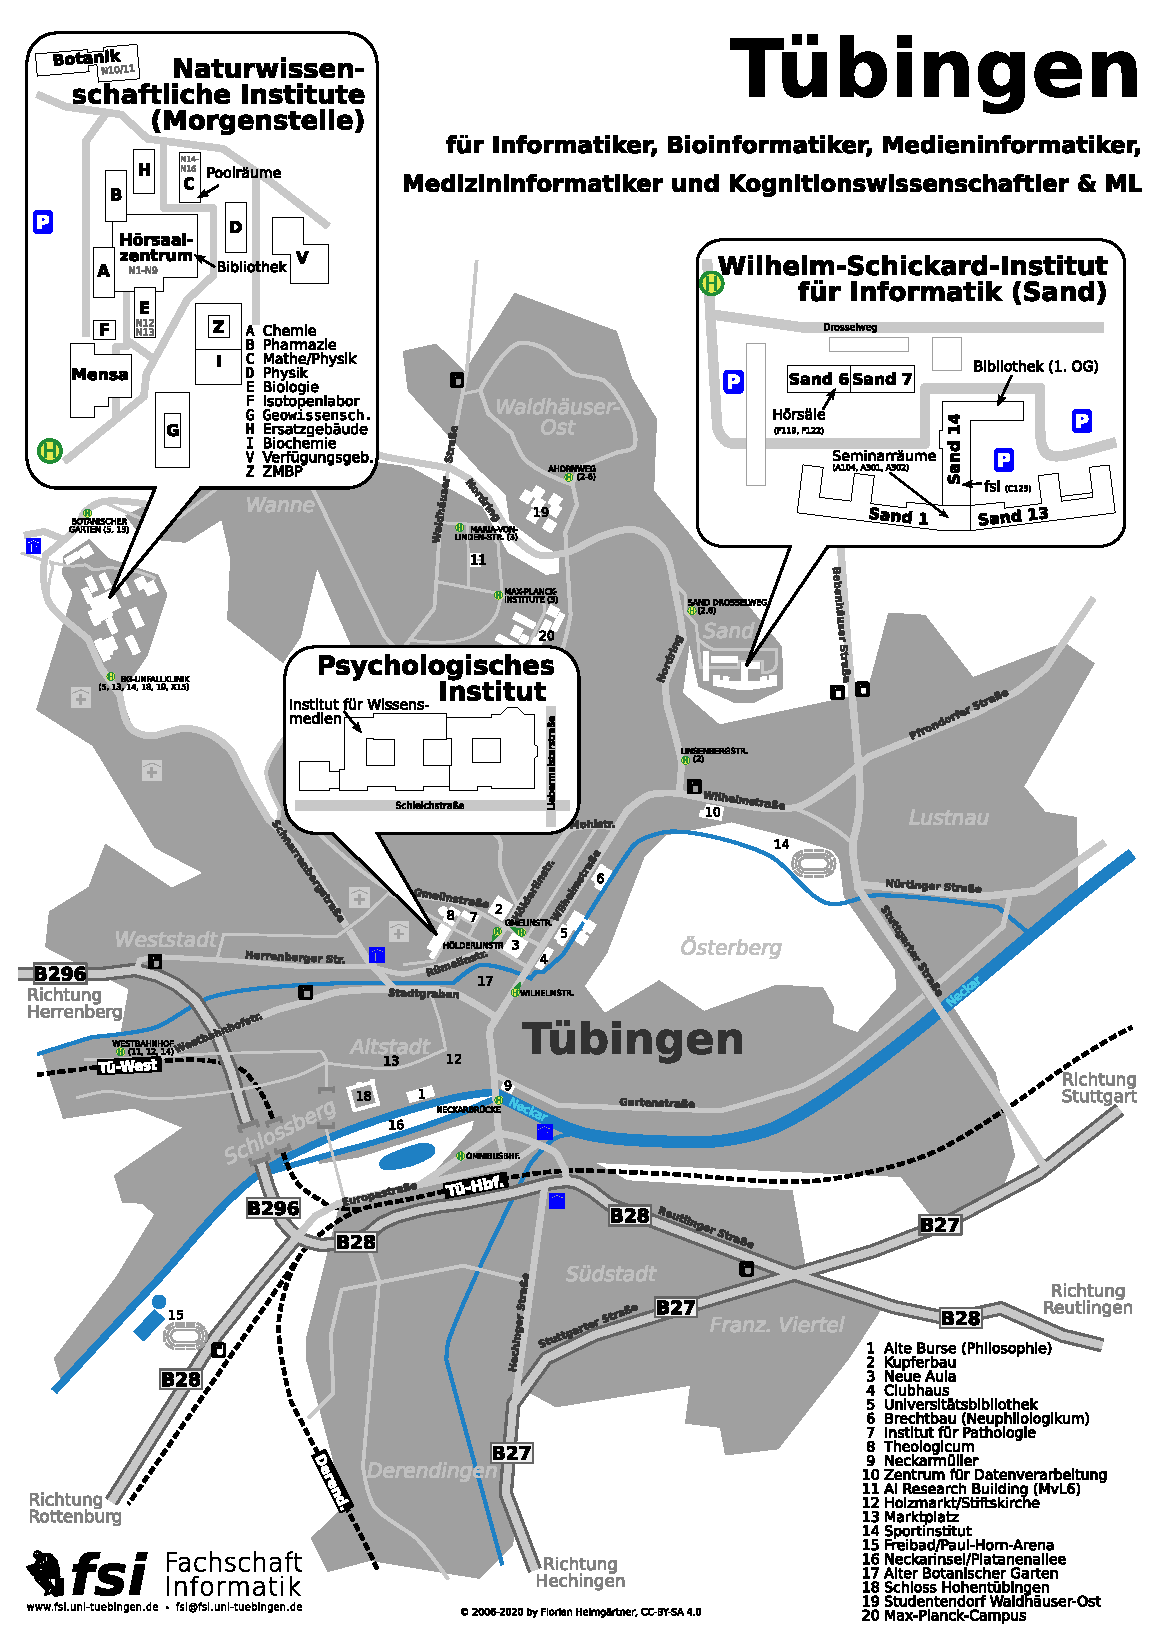
\includepdf[delta=5mm 5mm]{pdf/stadtplan.pdf}
  \end{letter}
\end{document}
